\documentclass[conference,12pt]{IEEEtran}

\usepackage[tight,footnotesize]{subfigure}

\usepackage{algorithmic}
\usepackage[boxed]{algorithm}

\ifCLASSINFOpdf
  \usepackage[pdftex]{graphicx}
  \graphicspath{{./images/}}
\else
\fi

\hyphenation{op-tical net-works semi-conduc-tor}

\begin{document}
	
\title{SDP Report 1}

\author{\IEEEauthorblockN{Marc Howarth}
\IEEEauthorblockA{Group 12 - Robot Unicorn Defenders}}
	
\maketitle

\IEEEpeerreviewmaketitle
	
\section{Introduction}
At our first group meeting, we decided to split into three different sub-teams. These were: motion and behaviour, robot construction and, vision. I joined the motion and behaviour team, with Roberto and Juozas, as I felt my strengths lay in the mathematical aspects of the project. 
	
\section{leJOS}
The firmware that comes pre-installed on the Lego Mindstorms NXT is somewhat limited and so Calum and myself researched which programming languages could be used instead. We eventually decided that leJOS\footnote{http://lejos.sourceforge.net/} would be a good choice. Previous years had used leJOS for their projects, there were multiple leJOS tutorials found online with relative ease and, taking into consideration the skill set of our group, Java was a popular choice.

With leJOS simply installing a Java virtual machine, it allows the robot to be programmed using Java. Installing leJOS was hassle free, and it didn't take us long to compile, transfer and execute our own programs.

	
\section{Bluetooth}	
The majority of the preliminary work has been done on my laptop because the DICE machines weren't immediately set up with leJOS. Whilst connecting to the NXT brick was working fine via USB, establishing a Bluetooth connection proved a little harder. After changing some settings on my laptop and installing additional drivers, we managed to successfully pair the two device. It was now possible to upload our own programs using only Bluetooth. The next step was to create a data stream between my laptop and the NXT brick inevitably such that commands could be sent to the robot over a permanent Bluetooth connection.

We now had the basis of a simple client-server model. The laptop would act as a server whilst the NXT brick would be the client waiting for commands to be send from the server. It was decided to only have the data stream going one way. This was because the only information that would need to be sent back to the server would be from the sensors. The program running on the NXT brick will be designed to handle the information from the sensors without having to send any information to the server. The flow of information can be seen in Figure \ref{fig:dataFlow}.

Now that the connection was established I installed a program onto the NXT brick that would infinitely loop until a command was received. Then, there was a series of if statements that would only run when a specific command was given. The command "123" moved the robot forwards and the command "321" send the robot backwards. This gave a good demonstration on how the code could be structured with obvious room for expansion. Pseudocode for this process can be seen in Algorithm 1 and 2.

\section{First Milestone}
In preparation for the first milestone as defined in the Course guide \footnote{http://www.inf.ed.ac.uk/teaching/courses/sdp/sdp\-course\-guide.pdf} our robot must demonstrate that it can perform a legal penalty kick. 

To strike the ball, a kicker was made by attaching long pieces of Lego to a motor. The motor was mounted high in the robot so that as much momentum and force could be gained for hitting the ball. The code needed for striking the ball required a bit of trial and error to ensure that the motor runs for the perfect amount of time.

\pagebreak

\section{Appendix}

\begin{figure}[htp]
\begin{center}
%\leavevmode
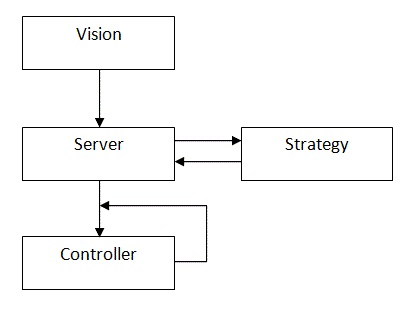
\includegraphics[width=0.4\textwidth] {flowchart.jpg}
\end{center}
\caption{Flow of data through the system}
\label{fig:dataFlow}
\end{figure}

\begin{algorithm}
\label{fig:codeClient}
\caption{Code running on the NXT brick}
\begin{algorithmic}[1]
\STATE connecthBluetooth()
\STATE establishDataStream()
\WHILE {true}
	\IF{command == 1} 
		\STATE kick()
	\ELSIF{command == 123}
		\STATE goForwards()
	\ELSIF{command == 321}
		\STATE goBackwards()
	\ELSE
		\STATE error
	\ENDIF
\ENDWHILE
\end{algorithmic}
\end{algorithm}

\begin{algorithm}
\label{fig:codeServer}
\caption{Code running on the server}
\begin{algorithmic}[1]
\STATE openServer("Roboto","00:16:53:0b:b5:a3")
\STATE sendCommand(123)
\STATE sendCommand(321)
\STATE sendCommand(1)
\STATE closeServer()
\end{algorithmic}
\end{algorithm}
	
\end{document}